\section{Website Prototype}\label{sec:prototype}
In order to get a better idea of how the website should look like, various prototypes were drawn.
As they are prototypes, they are by no means a representation of the final product, but more of a source of inspiration and brainstorming, to consider when developing the website.
Throughout this section, prototype sketches for different parts of the website, is presented, explained, and discussed.
Our primary inspiration is based on the current website for \bycykelwithoutspace \citep[misc:aalborgbycykelMain].

\begin{figure}[h]
	\centering
	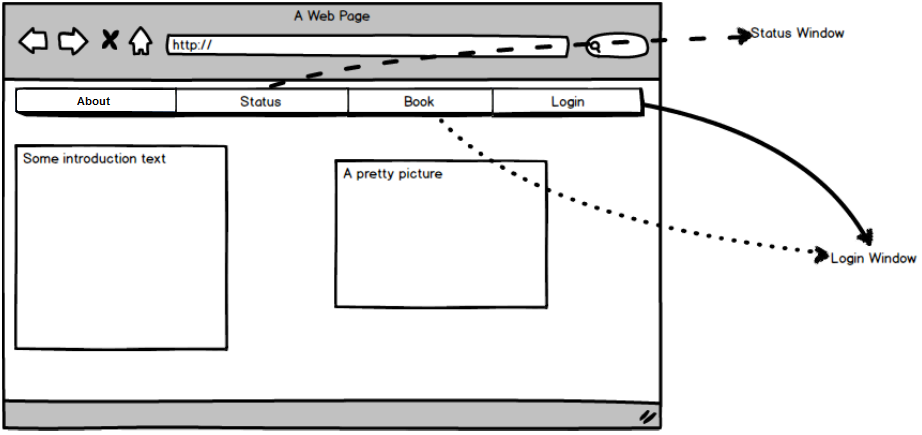
\includegraphics[scale=0.6]{design/prototype-about}
	\caption{About page.}\label{fig:prototype-about}
\end{figure}

First, we take a look at \figref{fig:prototype-about}.
This illustration presents a draft of the about page, it is structured as a standard about page with some description of the organisation behind the website.
What is more interesting to see in this illustration is the first draft of the menu bar.
The menu bar consists of links to about, status, book, and login, each of which have their page(s) illustrated hereafter.

\begin{figure}[h]
	\centering
	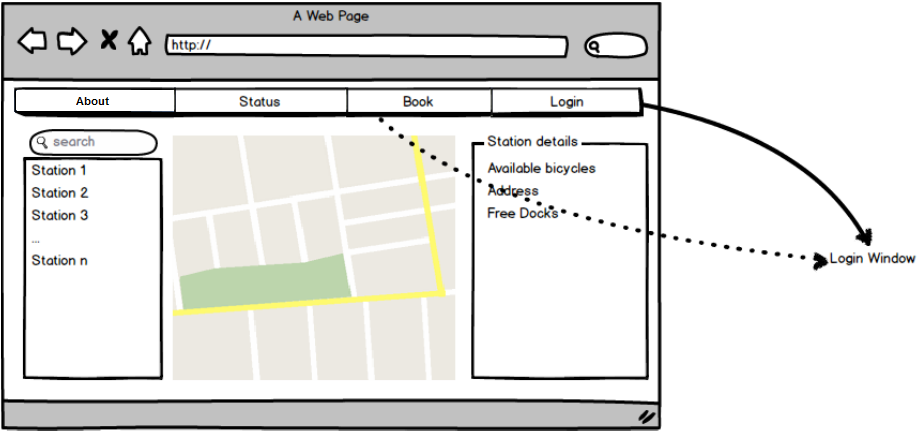
\includegraphics[scale=0.6]{design/prototype-status}
	\caption{Status page.}\label{fig:prototype-status}
\end{figure}

Next is a presentation of the status page, see \figref{fig:prototype-status}.
The main idea here is that the status page should be easily accessible and is what should be shown when navigating to the homepage.
The reason for this is that the status page should easily be able to give you an overview of the status of each station.
As can be seen from the illustration, this station detail can be found by selecting a station from a table, searching for it, or selecting the station on a map.
When a station is selected, details will be shown for it, which can be useful to see if available bicycles exist at the station.
In many ways, the status page is similar to the booking page, which will be presented hereafter.

\begin{figure}[h]
	\centering
	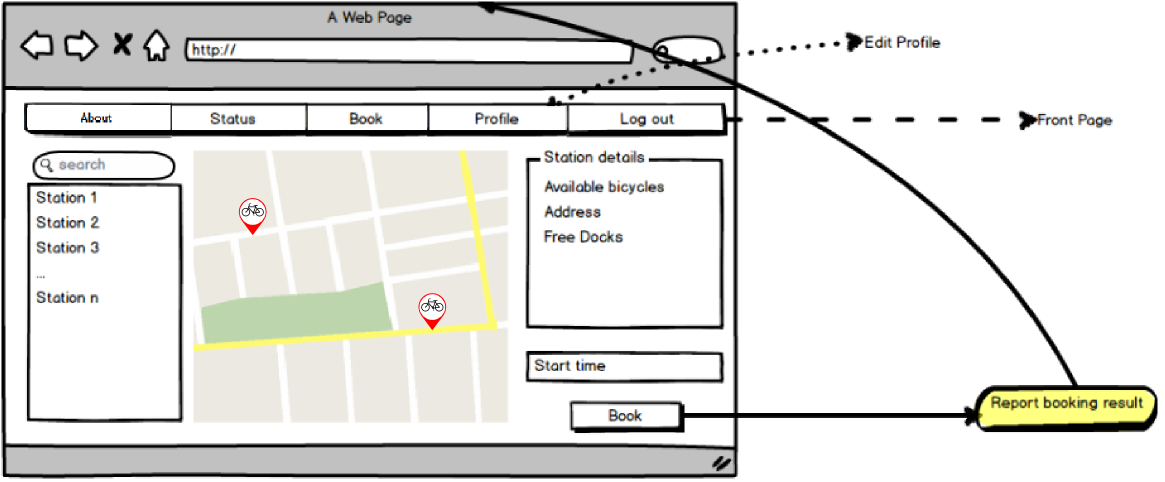
\includegraphics[scale=0.6]{design/prototype-booking}
	\caption{Booking page.}\label{fig:prototype-book}
\end{figure}

For an illustration of the booking page, see \figref{fig:prototype-book}.
The booking page can only be navigated to if you are logged in, if not you are redirected to a login page.
The booking page is otherwise the same as the status page, except you are able to book a bicycle at a given time.
To make a booking, you would login to the website and navigate to the booking page.
Thereafter you would select a station where you want to book a bicycle and select start time, which is the time you expect to retrieve the bicycle.
When you then click \textit{Book}, the booking result will be handled and registered in the system if valid.

Prototype pages also exist for the profile login and management, but has been omitted here, as these pages are very standard pages.
In that meaning one page being a login form and another page being a form with some fields to edit your password, phone, and email.
What is interesting though, is that you can access your booking history page through the profile page.

\begin{figure}[h]
	\centering
	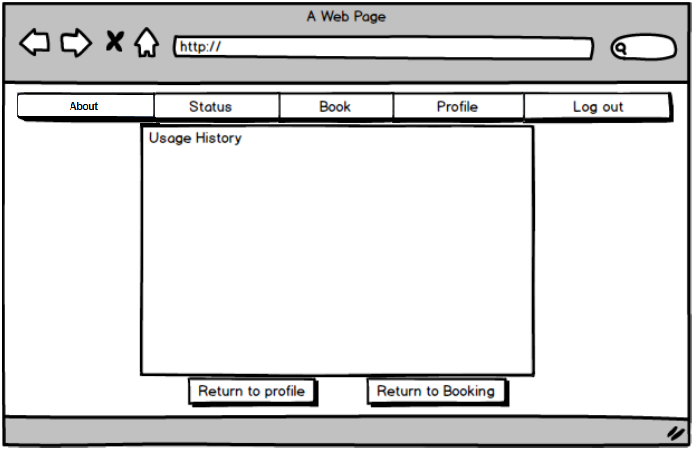
\includegraphics[scale=0.6]{design/prototype-usage-history}
	\caption{Booking history page.}\label{fig:prototype-usage-history}
\end{figure}

The booking history page can be seen in \figref{fig:prototype-usage-history} and will show your whole booking history.
It is generally reassuring information that can show the user that their bookings have been handled correctly by the system, to support the user that is afraid that the system have not registered their action. \fxwarning{Skal vi have en kilde på det?}
Furthermore, sometimes you see webshops provide purchase histories, and you can for this page consider a booking a metaphor for a purchase.

This ends the description of the prototypes for the system, and is what we first had in mind before implementing the system, and as of such you will later see some parts of this used for the implemented system.